\documentclass{article}
\usepackage[utf8x]{inputenc}

\usepackage{xcolor}
% \AddToHook{shipout/before}{%
%   \ifodd\value{page}
%     \pagecolor{blue!10!white}% Odd page colour (light blue)
%   \else
%     \pagecolor{red!10!white}% Even page colour (light red)
%   \fi
% }


\usepackage{geometry}
\geometry{letterpaper, margin=1in}

\providecommand{\tightlist}{%
  \setlength{\itemsep}{0pt}\setlength{\parskip}{0pt}}

\usepackage{adjustbox}
\usepackage[hyphens]{url}
\usepackage{lineno,hyperref}
\modulolinenumbers[5]

%% APA style
\usepackage{graphicx}
\usepackage{caption}

\definecolor{dimgray}{rgb}{0.41, 0.41, 0.41}
\definecolor{aureolin}{rgb}{0.99, 0.93, 0.0}
\definecolor{aqua}{rgb}{0.0, 1.0, 1.0}
\definecolor{deepmagenta}{rgb}{0.8, 0.0, 0.8}
\definecolor{almond}{rgb}{0.94, 0.87, 0.8}
\usepackage{pagecolor}
\usepackage{afterpage}

\begin{document}
\pagestyle{empty}
\thispagestyle{empty}
\pagecolor{dimgray!30}

\begin{figure}[h]
\begin{adjustbox}{minipage=[c]{\textwidth-10mm},margin= 5mm 35mm 5mm 27mm, frame=1pt, bgcolor=almond,env=center}%
%\begin{adjustbox}{varwidth=\textwidth,bgcolor=almond,margin=3mm {\abovecaptionskip} 3mm 3mm, frame=1pt }
\begin{center}
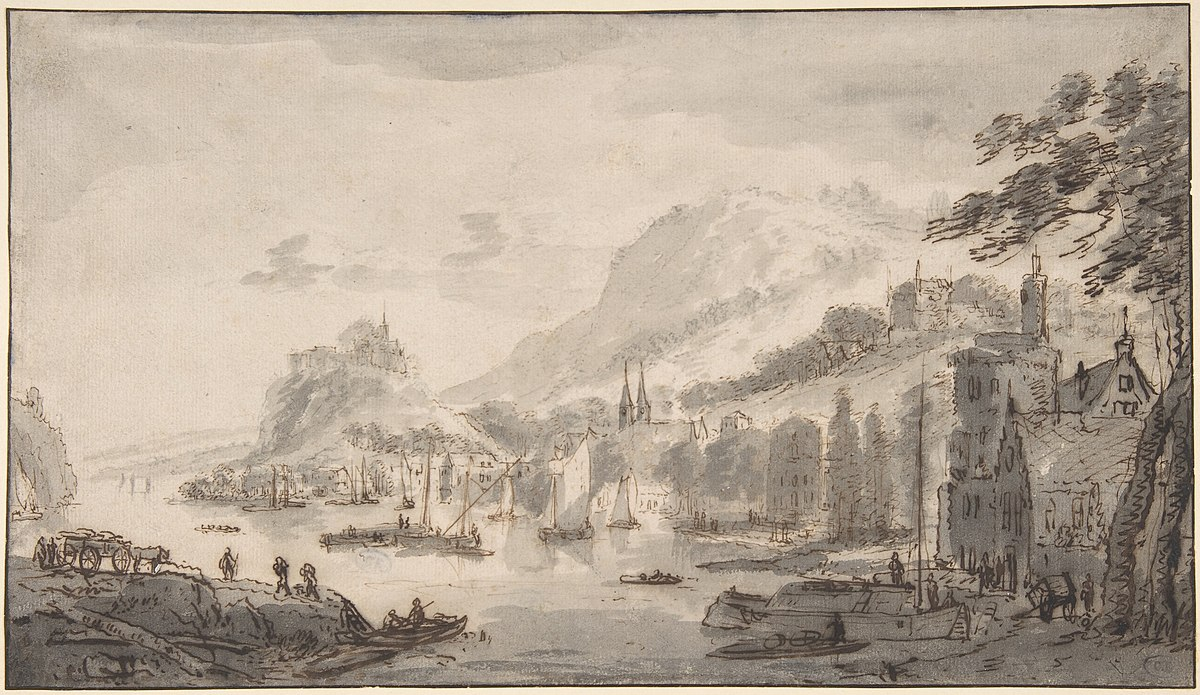
\includegraphics[trim=0mm 0mm 0mm 0mm, clip,width=.7\paperwidth]{water_town.jpg}
\end{center}

\begin{center}
\begin{minipage}[t]{0.7\paperwidth}

\medskip
{\huge Designer}
\bigskip

\Large\raggedright
\textbf{Context} When developing a vision of the future.\newline
\textbf{If} people start to form a solution BUT we don’t connect it with our existing knowledge, then it’s likely to be fragile;\newline
\textbf{Then} use words like “\emph{therefore}” to describe the solution in terms of other known solutions.
\end{minipage}
\end{center}
\caption*{Town by a Large Body of Water, drawing, Abraham Rademaker (MET, 1975.131.160). Public domain, via Wikimedia Commons.\newline
\url{https://commons.wikimedia.org/wiki/File:Town_by_a_Large_Body_of_Water_MET_DP800608.jpg}}
\end{adjustbox}
\end{figure}

\end{document}